\documentclass[type = bachelor]{whu-thesis}
\usepackage{textcomp,mathcomp}
\usepackage{siunitx}
\usepackage{chemfig}
\usepackage{graphicx}

\whusetup
  {
    info               =
      {
        title          = {金刚石氮-空位色心的\\电荷态调控和性质表征},
        title*         = {Modulation of Charge States and Characterization of Properties\\ in Nitrogen-Vacancy Centers of Diamond},
        student-number = {2020302192129},
        school         = {弘毅学堂},
        author         = {邹迪玮},
        author*        = {Diwei Zou},
        subject        = {学科},
        major          = {微电子科学与工程},
        advisor        = {周利 , 副教授;孙启超 , 研究员},
        direction      = {研究方向},
        date           = {2024/5},
        keywords       = {关键词 1 , 关键词 2 , 关键词 3 , 关键词 4 , 一个非常非常,非常非常长——的关键词 5},
        keywords*      = {key word 1 , key word 2 , key word 3 , key word 4 , {and a very very, very very long key word---the key word 5}},
      },
    style              =
      {
        graphics-path  = {{figures/}{data/}},
        list-of-figures,
        list-of-tables,
      },
    element            =
      {
        innovation     = {pages/innovation},
        abstract       = {pages/abstract},
        abstract*      = {pages/enabstract},
        bibliography   = {ref/refs_2}
      }
  }
\begin{document}


% Chapter 2

\chapter{NV Center电荷态动力学的理论原理}

\section{NV Center的电荷态}
因为NV Center电荷态的一些最基本的性质和特征已经在第一章中有所分析,所以本章主要聚焦于NV Center电荷态动力学的理论原理,也就是本文后续实验中所主要研究的对象和内容。本文主要研究的对象是NV Center的负电状态NV$^-$和中性状态NV$^0$,而NV Center的正电状态NV$^+$由于其电子结构的特殊性,其电荷态动力学的研究相对较少,所以本文不做过多的讨论\cite{schreyvogel2016active}。

\subsection{NV Center电荷态的荧光光谱}

在第一章的图 1.7中,我们可以看到NV Center的不同电荷态的荧光发射光谱的特征。在NV Center的荧光光谱中,我们可以看到NV$^-$和NV$^0$的荧光峰分别位于$637$ nm和$575$ nm处,。在实验中,我们可以通过测量NV Center的荧光光谱来判断其电荷态,从而可以对NV Center的电荷态进行观测和表征。

在NV$^-$和NV$^0$的两个光谱曲线中,可以看到声子边带(phonon sidebands, PSB)的作用强度都比ZPL的强度更高,这个过程可以用利用基于Born-Oppenheimer近似和Franck-Condon原理的Huang-Rhys模型来进行简单地描述,即在分子或晶体中,当电子从其基态激发到一个激发态时,会导致与电子激发相关的振动模式被激发。这些振动模式的能级通常称为 "振动激发" 或 "振动副态",而Huang-Rhys 模型用来描述这些振动激发的分布和对电子激发的影响,如图 \ref{fig: Franck-Condon} \cite{zou2023influence}。在这个模型之中,Huang-Rhys因子$S$决定了晶体结构在基态和激发态之间平衡态位置的差异,这个差异体现了吸收和发射光谱之间的斯托克斯能量位移$E_{Stokes}$。斯托克斯能量唯一和Huang-Rhys因子之间的关系取决于温度,因为基态和能动能级之间的能量差异导致的光谱线会随着温度的升高而展宽,一个比较粗略的计算式如下\cite{de2015resolving}: 
\begin{equation}
  S = (\frac{E_{Stokes}}{2\hbar \omega}+\frac{1}{4})±\frac{1}{4}
\end{equation}
其中$\hbar \omega$代表着缺陷周围晶体的平均声子能量。

\begin{figure}
  \centering
  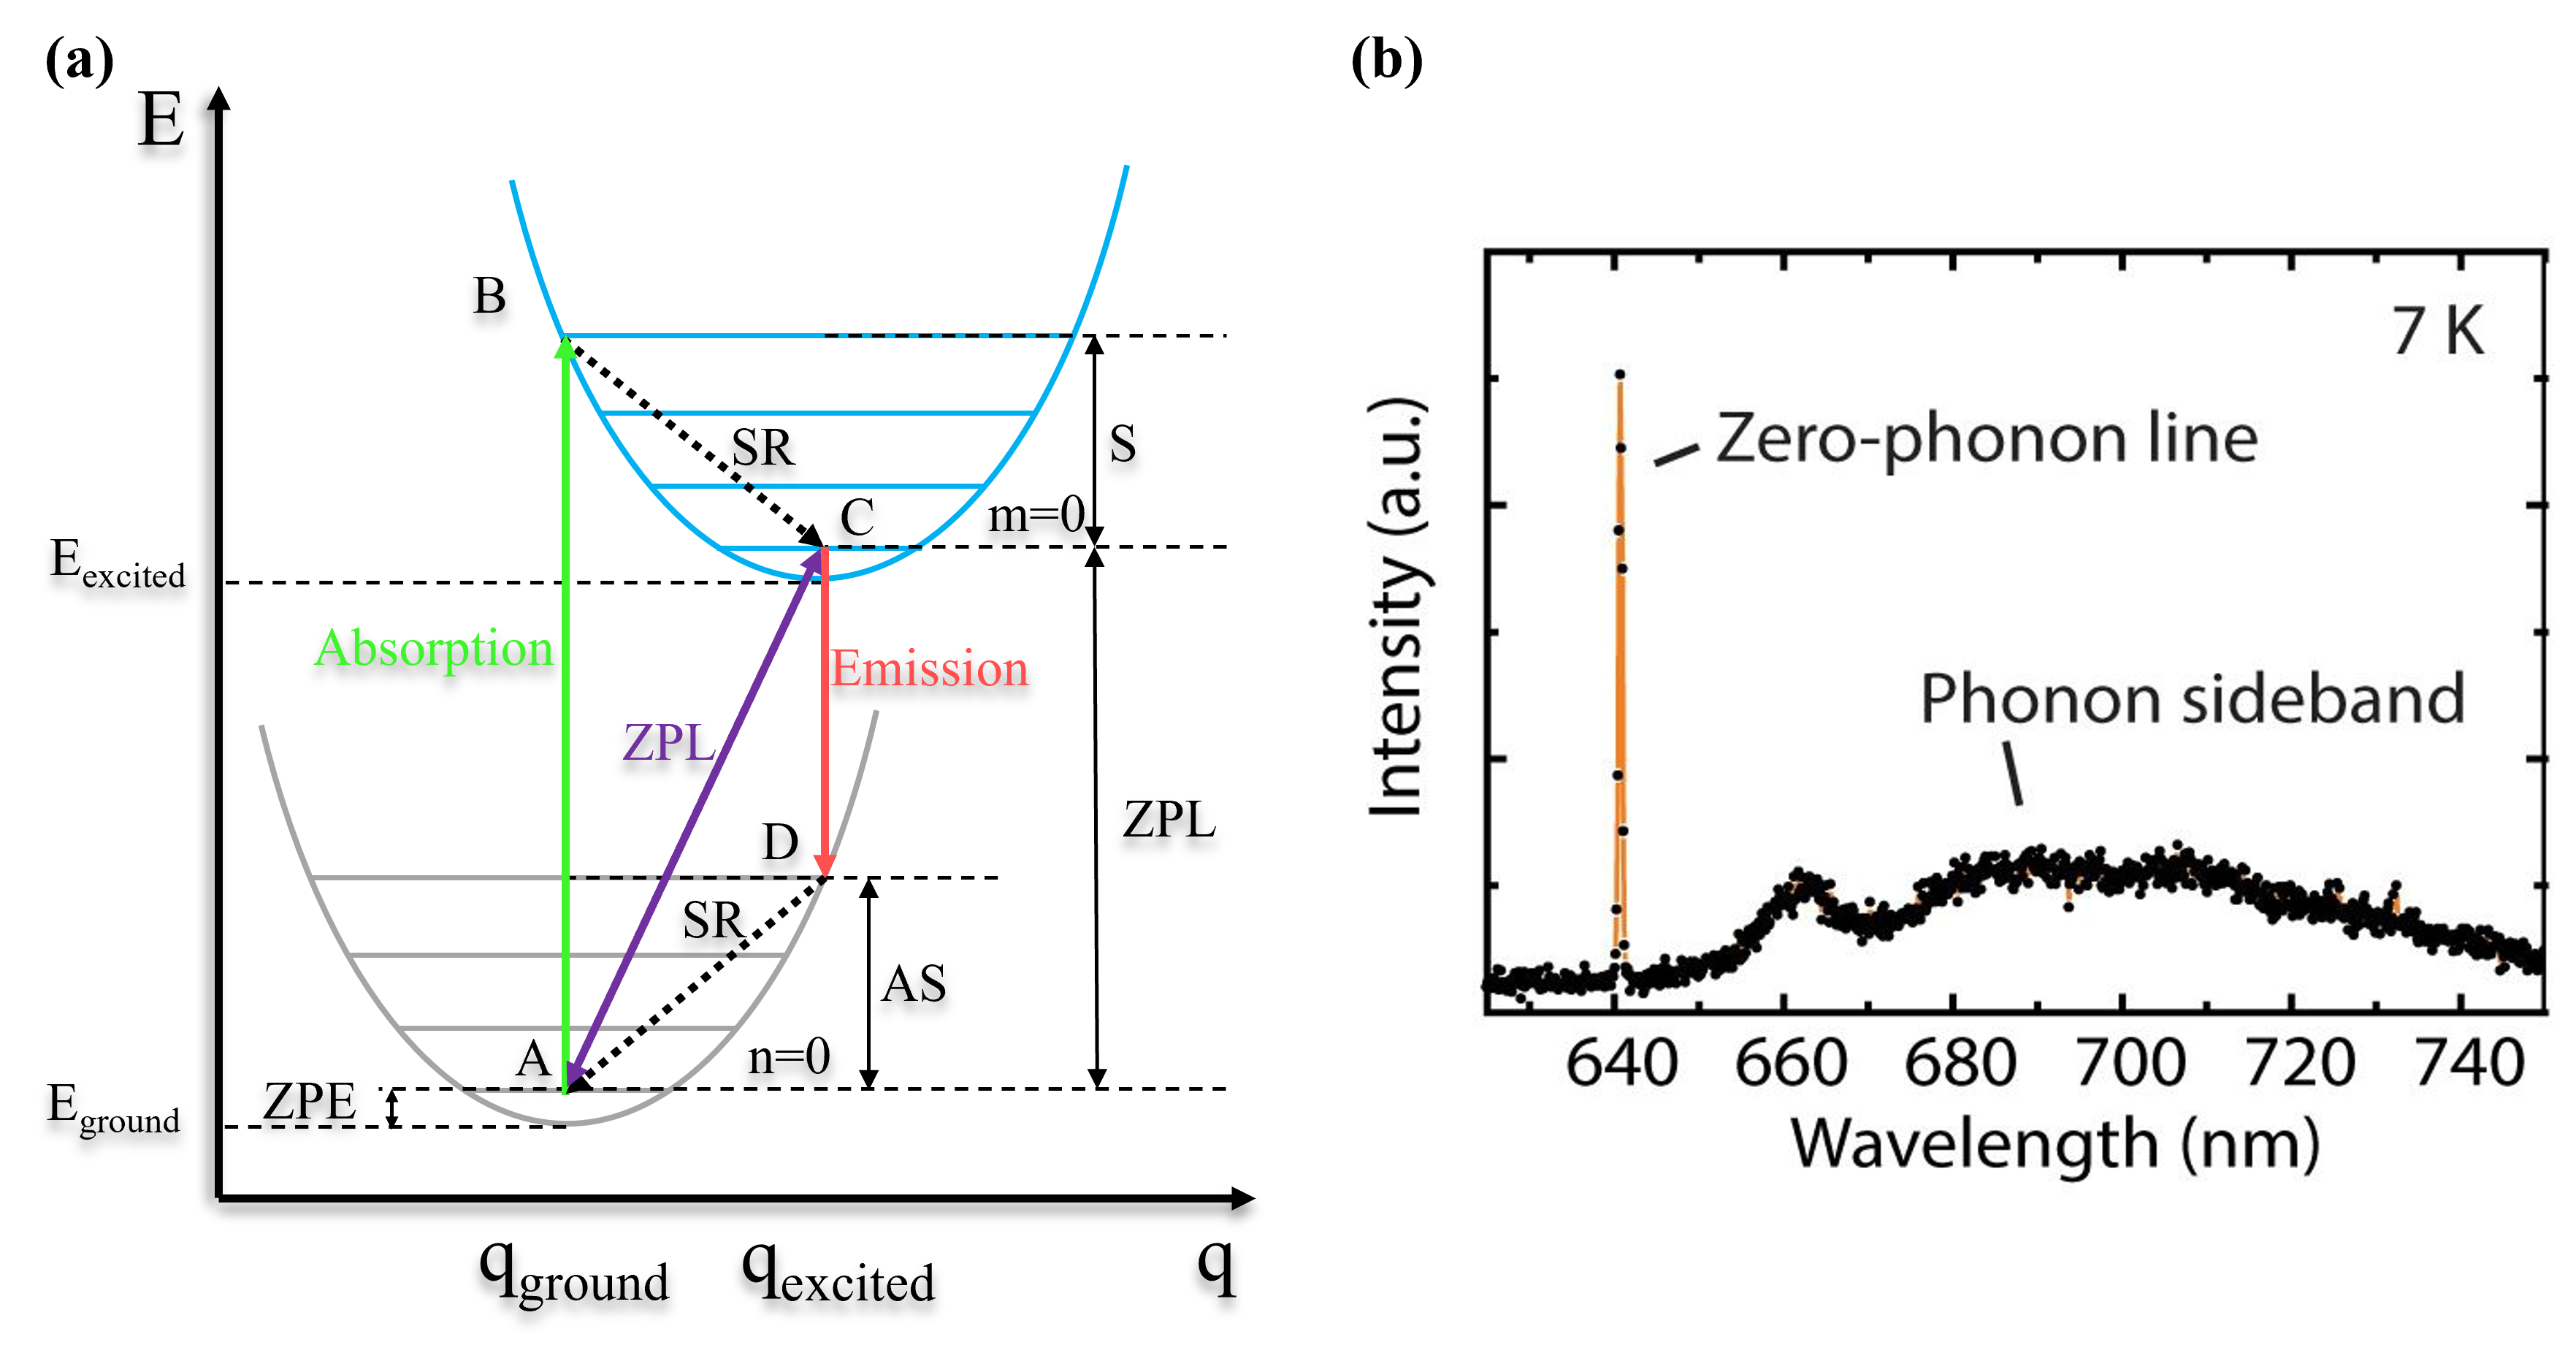
\includegraphics[width=1.0\textwidth]{figures/Chapter 2/Franck-Condon.png}
  \caption[基于Born-Oppenheimer近似和Franck-Condon原理的Huang-Rhys模型示意图]{基于Born-Oppenheimer近似和Franck-Condon原理的Huang-Rhys模型示意图,展示了体系能量(E)和晶体结构坐标(q)的关系。纵轴上的E$_{ground}$和E$_{excited}$分别代表着基态和激发态准抛物线近似能量面的最低能量值,横轴上的q$_{ground}$和q$_{excited}$代表着基态和激发态晶体结构的平衡位置}
  \label{fig: Franck-Condon}
\end{figure}


\subsection{各节二级标题}
你是内容

\subsubsection{各节三级标题}
他是内容

\paragraph{四级标题}
内容内容

\subparagraph{五级标题}
内容内容

\section{字体样式}
宋体\quad \textbf{粗体}\quad \textit{斜体}\quad \textbf{\textit{粗斜体}}。

{\heiti 黑体\quad \textbf{粗体}\quad \textit{斜体}\quad \textbf{\textit{粗斜体}}}。

{\fangsong 仿宋\quad \textbf{粗体}\quad \textit{斜体}\quad \textbf{\textit{粗斜体}}}。

{\kaishu 楷书\quad \textbf{粗体}\quad \textit{斜体}\quad \textbf{\textit{粗斜体}}}。

Serif\quad \textit{Italic}\quad \textbf{Bold}\quad \textbf{\textit{BoldItalic}}

{\sffamily Sans\quad \textit{Italic}\quad \textbf{Bold}\quad \textbf{\textit{BoldItalic}}}

{\ttfamily Mono\quad \textit{Italic}\quad \textbf{Bold}\quad \textbf{\textit{BoldItalic}}}

\end{document}